\section{Posició relativa de dos plans}

Donats dos plans $\pi: Ax + By + Cz + D = 0$ i $\pi': A'x + B'y + C'z + D' = 0$, la posició relativa es determina comparant els coeficients:

\begin{table}[H]
\centering
\renewcommand{\arraystretch}{1.25}
\begin{tabularx}{\textwidth}{lc>{\raggedright\arraybackslash}X}
\toprule
Plans coincidents & Plans paral\textperiodcentered{}lels & Plans secants \\
\midrule
$\dfrac{A}{A'} = \dfrac{B}{B'} = \dfrac{C}{C'} = \dfrac{D}{D'}$ & $\dfrac{A}{A'} = \dfrac{B}{B'} = \dfrac{C}{C'} \neq \dfrac{D}{D'}$ & No hi ha proporcionalitat entre els coeficients. La intersecció és una recta $r$. \\
\bottomrule
\end{tabularx}
\end{table}

\begin{figure}[H]
\centering
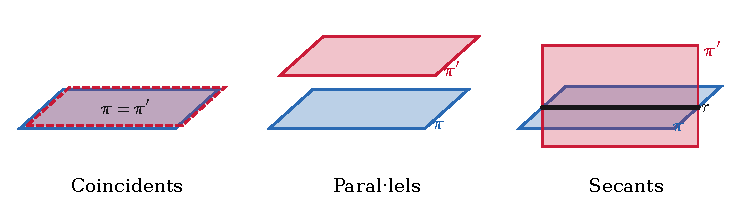
\includegraphics[width=372pt]{fig/m10_f19.pdf}
\caption{Posició relativa de dos plans: coincidents, paral\textperiodcentered{}lels i secants.}
\end{figure}

\section{Posició relativa de tres plans}

Amb tres plans, s'aplica el \textbf{Teorema de Rouché-Frobenius} sobre la matriu de coeficients $M$ i la matriu ampliada $M'$:

\begin{table}[H]
\centering
\renewcommand{\arraystretch}{1.25}
\begin{tabularx}{\textwidth}{lc>{\raggedright\arraybackslash}Xc}
\toprule
$\operatorname{Rg}(M)$ & $\operatorname{Rg}(M')$ & Posició relativa & Tipus \\
\midrule
1 & 1 & Tres plans coincidents & S.C.I \\
1 & 2 & Tres plans paral\textperiodcentered{}lels & S.I \\
2 & 2 & Tres plans secants a una recta $r$ comú & S.C.I \\
2 & 2 & Dos plans coincidents, l'altre secant als dos & S.C.I \\
2 & 3 & Prisma: plans secants dos a dos & S.I \\
2 & 3 & Dos plans paral\textperiodcentered{}lels, l'altre secant als dos & S.I \\
3 & 3 & Triedre: tres plans secants a un punt & S.C.D \\
\bottomrule
\end{tabularx}
\end{table}

\section{Posició relativa de recta i pla}

Per estudiar la posició de la recta $r$ i el pla $\pi$, es substitueixen les equacions paramètriques de $r$ a l'equació de $\pi$ i s'analitza el sistema resultant:

\begin{table}[H]
\centering
\renewcommand{\arraystretch}{1.25}
\begin{tabularx}{\textwidth}{>{\raggedright\arraybackslash}X>{\raggedright\arraybackslash}X>{\raggedright\arraybackslash}X}
\toprule
S.C.D & S.C.I & S.I \\
\midrule
$r$ i $\pi$ tenen un punt en comú (recta \textbf{secant} al pla) & $r$ està \textbf{continguda} en $\pi$ & $r$ i $\pi$ no tenen cap punt en comú (recta \textbf{paral\textperiodcentered{}lela} al pla) \\
\bottomrule
\end{tabularx}
\end{table}

\begin{figure}[H]
\centering
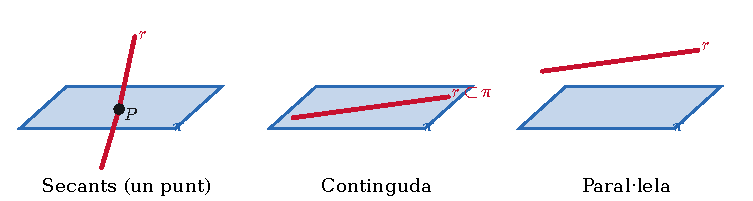
\includegraphics[width=372pt]{fig/m10_f20.pdf}
\caption{Les tres posicions relatives d'una recta i un pla.}
\end{figure}

\section{Posició relativa de dues rectes}

Expressades $r$ i $s$ com a intersecció de dos plans cadascuna, es forma un sistema de quatre equacions. Aplicant el TRF sobre la matriu $M$ i l'ampliada $M'$:

\begin{table}[H]
\centering
\renewcommand{\arraystretch}{1.25}
\begin{tabular}{lccc}
\toprule
S.C.D & S.C.I & S.I (1) & S.I (2) \\
\midrule
$\operatorname{Rg}(M) = 3 = \operatorname{Rg}(M')$ & $\operatorname{Rg}(M) = 2 = \operatorname{Rg}(M')$ & $\operatorname{Rg}(M) = 2 \neq \operatorname{Rg}(M') = 3$ & $\operatorname{Rg}(M) = 3 \neq \operatorname{Rg}(M') = 4$ \\
Rectes \textbf{secants} & Rectes \textbf{coincidents} & Rectes \textbf{paral\textperiodcentered{}leles} & Rectes que \textbf{s'encreuen} \\
\bottomrule
\end{tabular}
\end{table}

\subsection{Resum per vectors directors}

Donats els vectors directors $\vec u$ i $\vec v$ de $r$ i $s$, i el vector $\overrightarrow{PQ}$ entre un punt de cada recta:

\begin{itemize}
\item Si $\vec u = \lambda\vec v$ (vectors proporcionals, rectes paral\textperiodcentered{}leles o coincidents):
\begin{itemize}
\item $\overrightarrow{PQ} = \mu\,\vec u \Rightarrow$ rectes \textbf{coincidents}
\item $\overrightarrow{PQ} \neq \mu\,\vec u \Rightarrow$ rectes \textbf{paral\textperiodcentered{}leles}
\end{itemize}
\item Si $\vec u \neq \lambda\vec v$ (vectors no proporcionals):
\begin{itemize}
\item $D(\vec u, \vec v, \overrightarrow{PQ}) = 0 \Rightarrow$ rectes \textbf{secants}
\item $D(\vec u, \vec v, \overrightarrow{PQ}) \neq 0 \Rightarrow$ rectes que \textbf{s'encreuen}
\end{itemize}
\end{itemize}

on $D(\vec u, \vec v, \overrightarrow{PQ})$ és el determinant format per les tres files $\vec u$, $\vec v$ i $\overrightarrow{PQ}$.

\section{Perpendicularitat}

\subsection{Plans perpendiculars}

Dos plans $\pi_1$ i $\pi_2$ amb vectors normals $\vec n = (A, B, C)$ i $\vec n' = (A', B', C')$ són perpendiculars si:

\begin{equation*}
\vec n\cdot\vec n' = 0 \;\Longrightarrow\; AA' + BB' + CC' = 0
\end{equation*}

\subsection{Recta i pla perpendiculars}

Una recta de vector director $\vec v = (V_1, V_2, V_3)$ és perpendicular al pla $Ax + By + Cz + D = 0$ si $\vec v$ és proporcional al vector normal $\vec n = (A, B, C)$:

\begin{equation*}
\vec v = k\,\vec n,\; k \neq 0 \iff \frac{V_1}{A} = \frac{V_2}{B} = \frac{V_3}{C}
\end{equation*}

\subsection{Rectes perpendiculars}

Dues rectes amb vectors directors $\vec v$ i $\vec u$ són perpendiculars si:

\begin{equation*}
\vec v\cdot\vec u = 0
\end{equation*}

\section{Projeccions ortogonals sobre un pla}

\subsection{Projecció ortogonal d'un punt sobre un pla}

El punt $P'$ és la \textbf{projecció ortogonal} de $P$ sobre el pla $\pi$ si $P'$ és el peu de la perpendicular a $\pi$ que passa per $P$. Es troba com la intersecció de $\pi$ amb la recta perpendicular a $\pi$ que passa per $P$.

\begin{figure}[H]
\centering
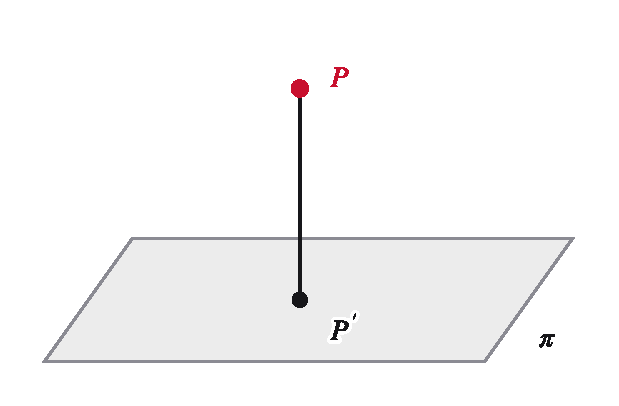
\includegraphics[width=297pt]{fig/m10_f21.pdf}
\caption{Projecció ortogonal del punt $P$ sobre el pla $\pi$: el punt $P'$ és el peu de la perpendicular.}
\end{figure}

\subsection{Projecció ortogonal d'una recta sobre un pla}

La projecció ortogonal d'una recta $r$ sobre un pla $\pi$ és la recta $r'$ que resulta d'intersectar $\pi$ amb el pla que conté $r$ i és perpendicular a $\pi$. Per a un segment $PQ$, es projecten els extrems $P$ i $Q$ per obtenir $P'$ i $Q'$.

\subsection{Projecció ortogonal d'un punt sobre una recta}

La projecció ortogonal del punt $P$ sobre la recta $r$ és el punt $P'$ intersecció de $r$ amb el pla perpendicular a $r$ que passa per $P$. El vector normal d'aquest pla coincideix amb el vector director de $r$.
